\documentclass{scrreprt}
\usepackage[english]{babel}
\usepackage[T1]{fontenc}
\usepackage{lmodern}
\usepackage{blindtext}
\usepackage[utf8]{inputenc}
\usepackage{siunitx} %For unit handling%
\renewcommand{\familydefault}{\sfdefault}
\newcommand{\unit}[1]{\ensuremath{\, \mathrm{#1}}}
\usepackage{amssymb, amsmath, cancel, ulem, graphicx, float, tabularx, multirow, bm}
\usepackage{amsmath}
\usepackage{caption}
\usepackage{subcaption}
\usepackage{tikz}
\newcommand*\circled[1]{\tikz[baseline=(char.base)]{
            \node[shape=circle,draw,inner sep=1pt] (char) {#1};}}

\setcounter{secnumdepth}{5}
\setcounter{tocdepth}{5}

\author{Urs Gerber\\09-921-156 \and Gian-Luca Mateo\\11-113-545}
\date{21th of March 2013}

\title{Airfoil in a wind channel}
\subtitle{Practical course report}

\begin{document}

\maketitle

\tableofcontents
\newpage

\chapter{Experiment: Airfoil in a wind channel}
\section{Introduction}
\subsection{Goal of the experiment}
The goal of this experiment is to determine the angle of attack where for a given airfoil the ratio of air drag to lift is optimal. Furthermore, the lift is to be calculated by measuring the pressure conditions on the surface of the airfoil.

\subsection{Theory}

\subsubsection{Bernoulli's Principle}
Bernoulli's Principle is a direct consequence of the \textbf{conservation of energy} and the \textbf{continuity equation}

\begin{equation}
\forall A : \rho \lvert \vec{v}\rvert A = p \dot{V} = const. \Longleftrightarrow \dot{V} = const.
\end{equation}
where $A$ is the cross section traversed by the fluid, $\vec{v}$ the fluid's velocity and $\dot{V}$ the volumetric flow rate through cross section $A$. Combining these two principles will yield Bernoulli's Principle:

\begin{equation}
\underbrace{\underbrace{p}_{\text{operating pressure}} + \underbrace{\rho g h}_{\text{geodesic pressure}}}_{\text{static pressure}} + \underbrace{\frac{1}{2} \rho \vec{v}^2}_{\text{dynamic pressure}} = const.
\end{equation}

\subsection{Circulation}
The \textbf{circulation} $\Gamma$ of a fluid around the profile of i.e. an air foil is defined as follows:
\begin{equation}
\Gamma = \oint_{\text{Profile}}\vec{v}\cdot\vec{dl}
\end{equation}

\subsection{Kutta–Joukowski theorem}
The magnitude of the boyant force $\vec{F_l}$ can be found using the \textbf{Kutta–Joukowski theorem} 
\begin{equation}
\lvert \vec{F_l}\rvert = b \rho \Gamma \lvert \vec{v}_\infty \rvert
\end{equation}

\subsection{Uncertainty analysis}
\paragraph*{Polar diagram}
\begin{equation}
\frac{F_l}{F_r} = \frac{m_h\cdot g}{m_v\cdot g} = \frac{m_h}{m_v} \doteq q
\end{equation}
\begin{equation}
\Longrightarrow s_q^2 = \frac{s_{\overline{m_h}}^2}{m_v^2} + \frac{s_{\overline{m_v}}^2 \cdot m_h^2}{m_v^4}
\end{equation}

\section{Experiment setup and execution}
\subsection{Used materials}
The materials used in this experiment are the following:
\begin{itemize}
\item A wind turbine (230V power supply, discrete control unit, steps from 0-9)
\item An airfoil with some holes from the surface to the sides (for measuring the pressure)
\item A balance which allows attaching a hinged airfoil
\item Some weights (1x200g, 1x100g, 1x50g, 2x20g, 1x10g, 1x5g, 2x2g, 1x1g)
\item A manometer (scale 0-17.5 mmWs, 0-16 m/s)
\item A prandtl tube
\end{itemize}

\begin{figure}[H]
        \centering
        \begin{subfigure}[b]{0.45\textwidth}
                \centering
                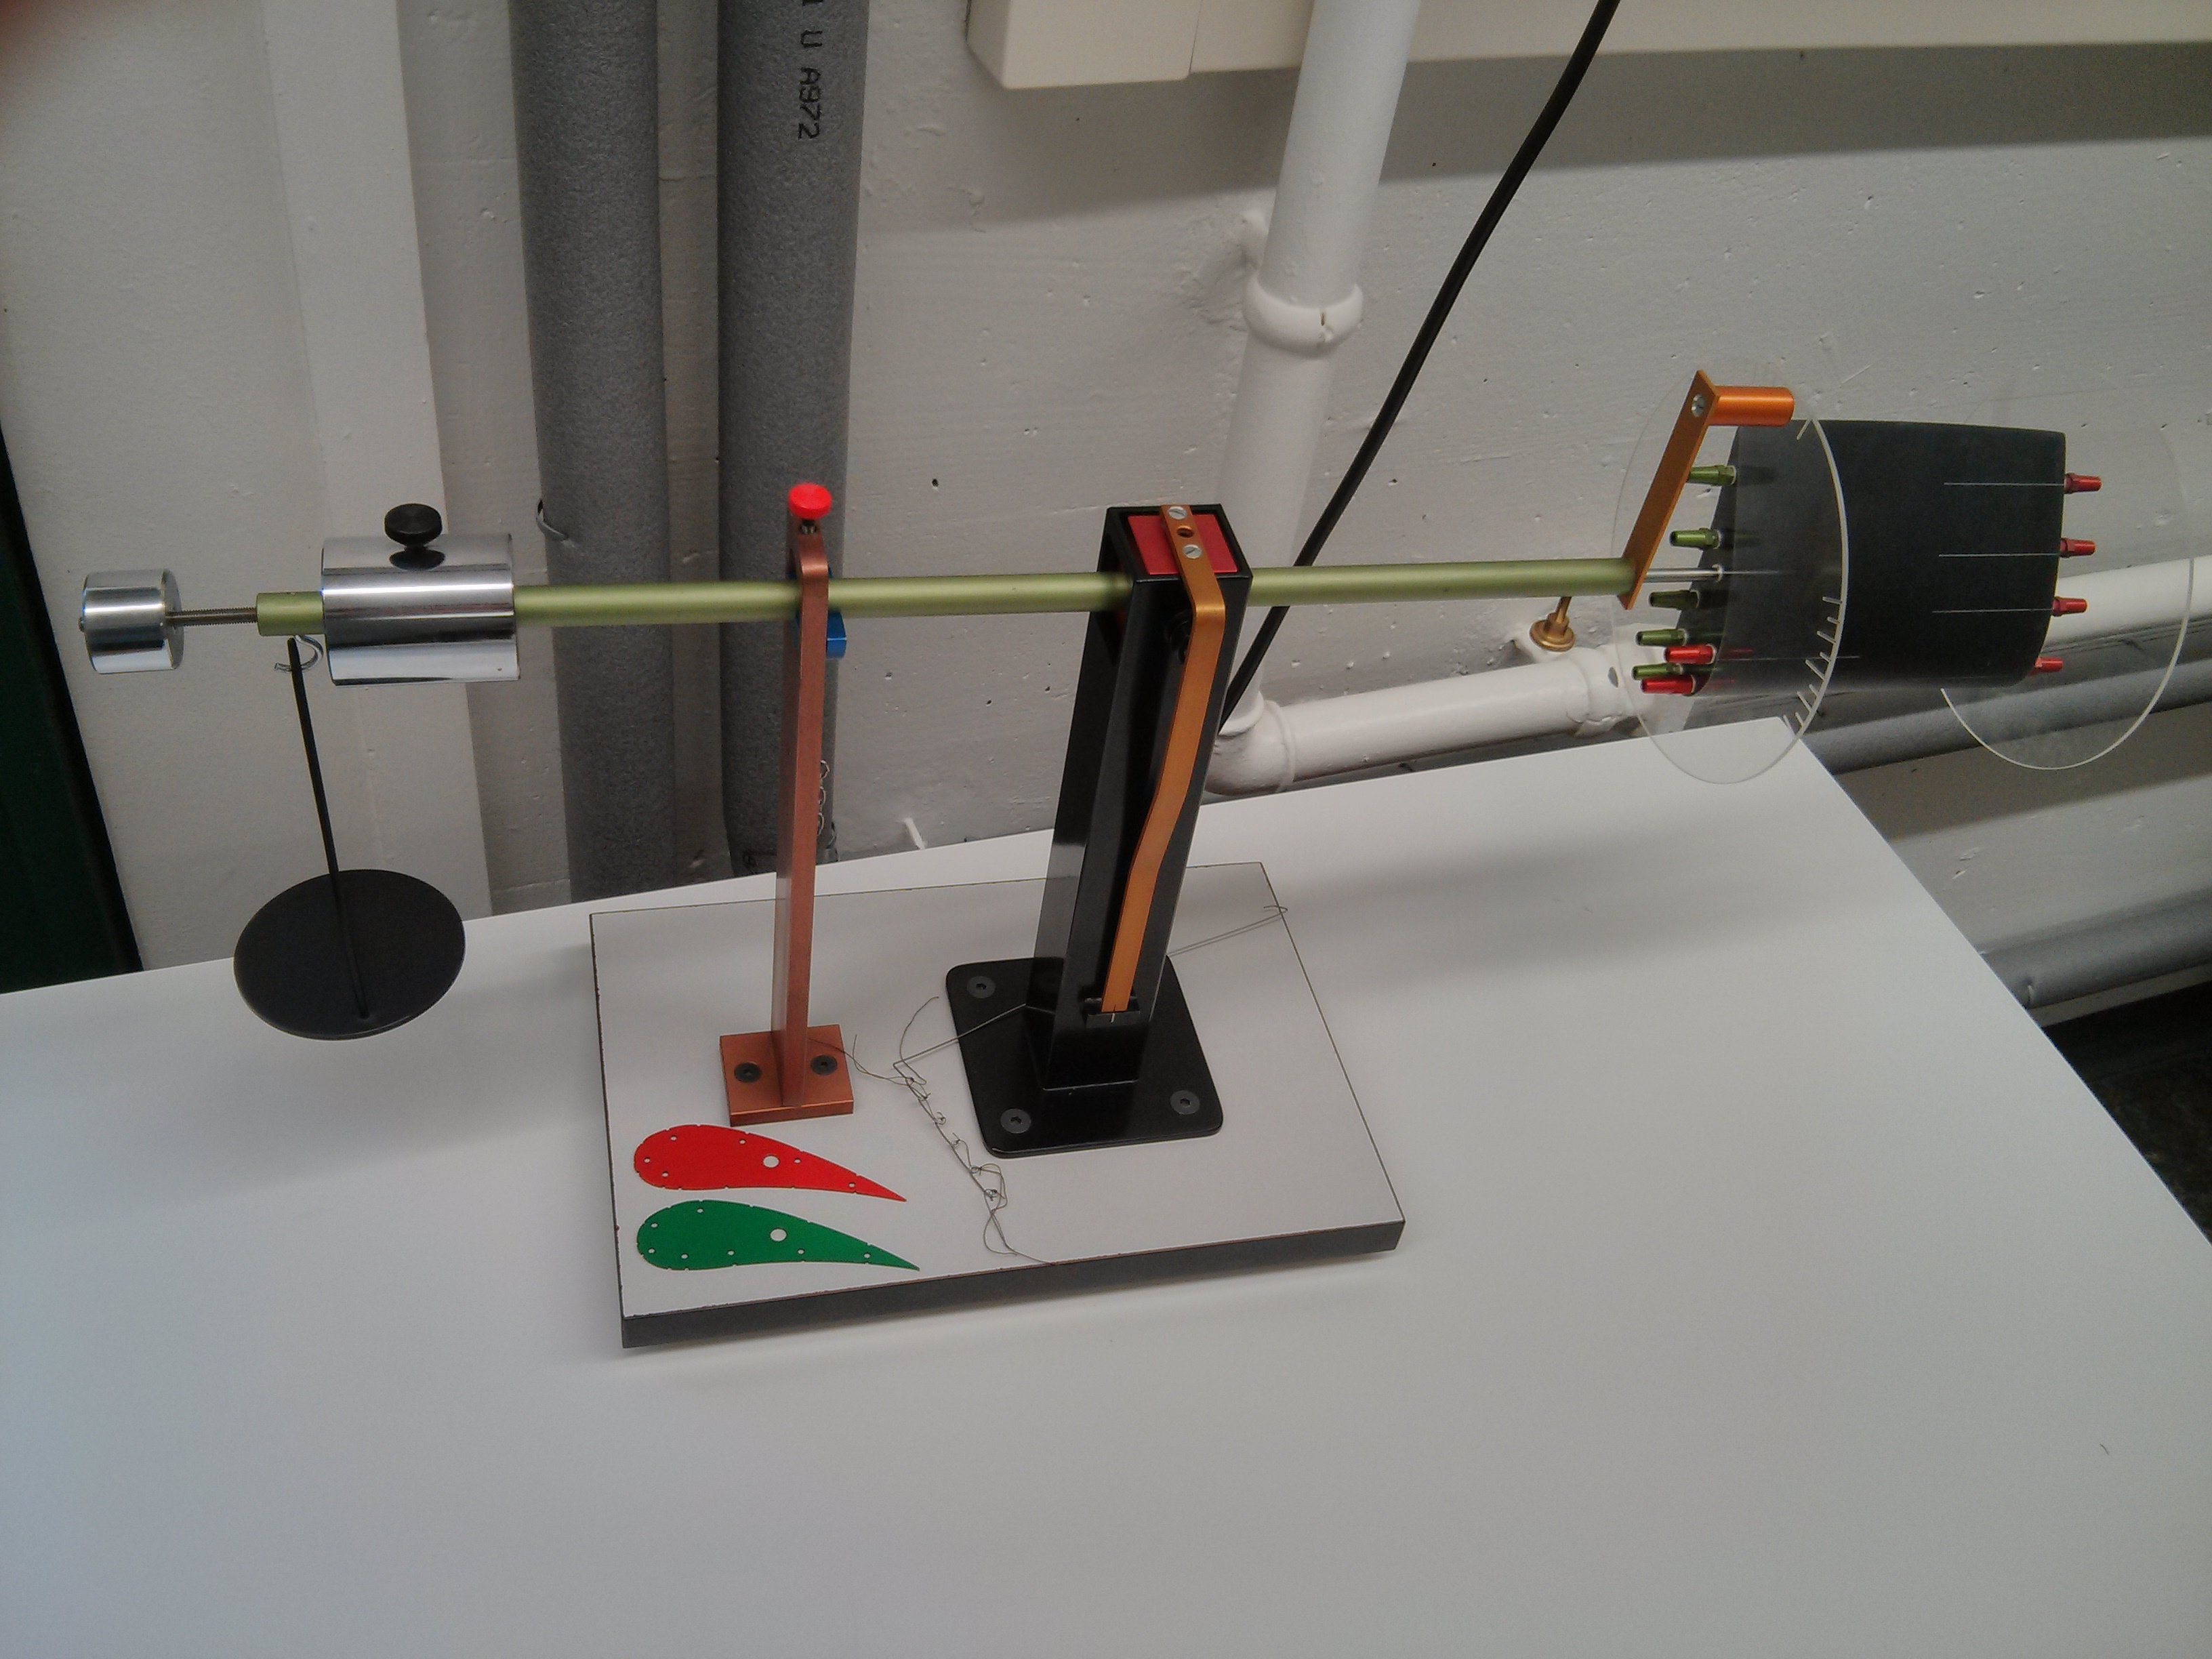
\includegraphics[width=\textwidth]{img/balance.jpg}
                \caption{Airfoil balance}
                \label{fig:balance}
        \end{subfigure}%
        ~
        \begin{subfigure}[b]{0.45\textwidth}
                \centering
                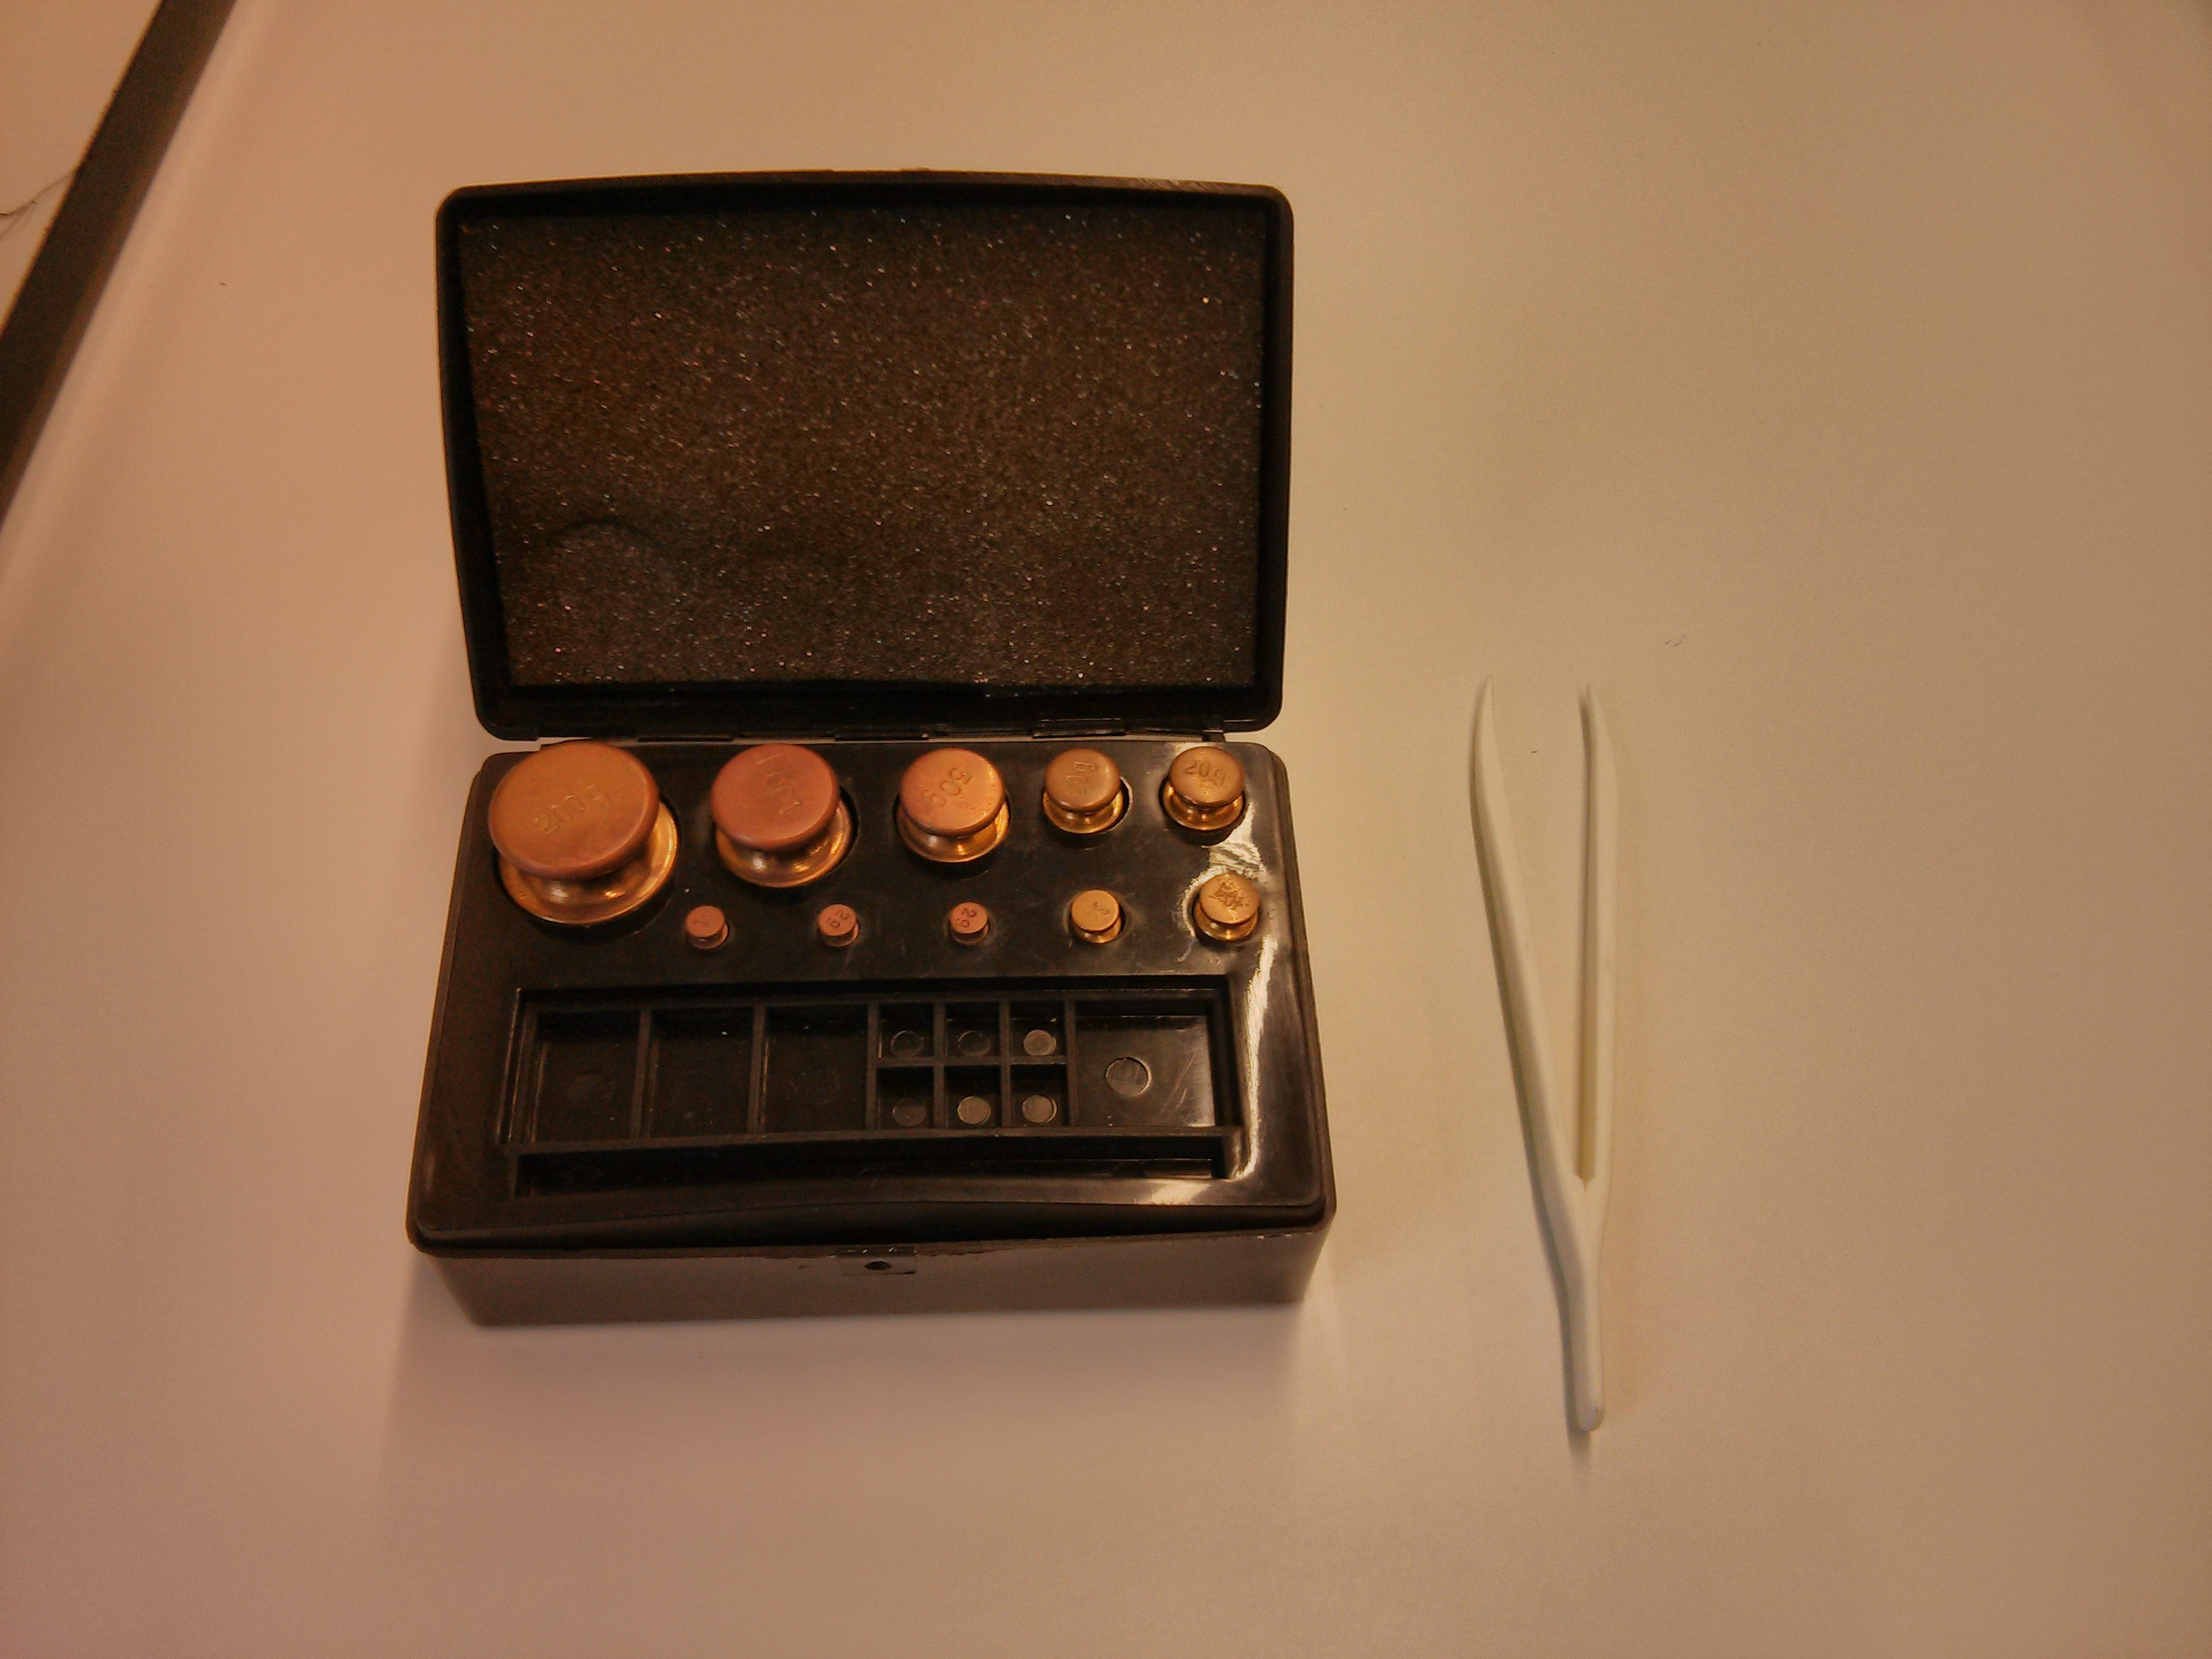
\includegraphics[width=\textwidth]{img/weights.jpg}
                \caption{Weights}
                \label{fig:weights}
        \end{subfigure}
          
        \begin{subfigure}[b]{0.45\textwidth}
                \centering
                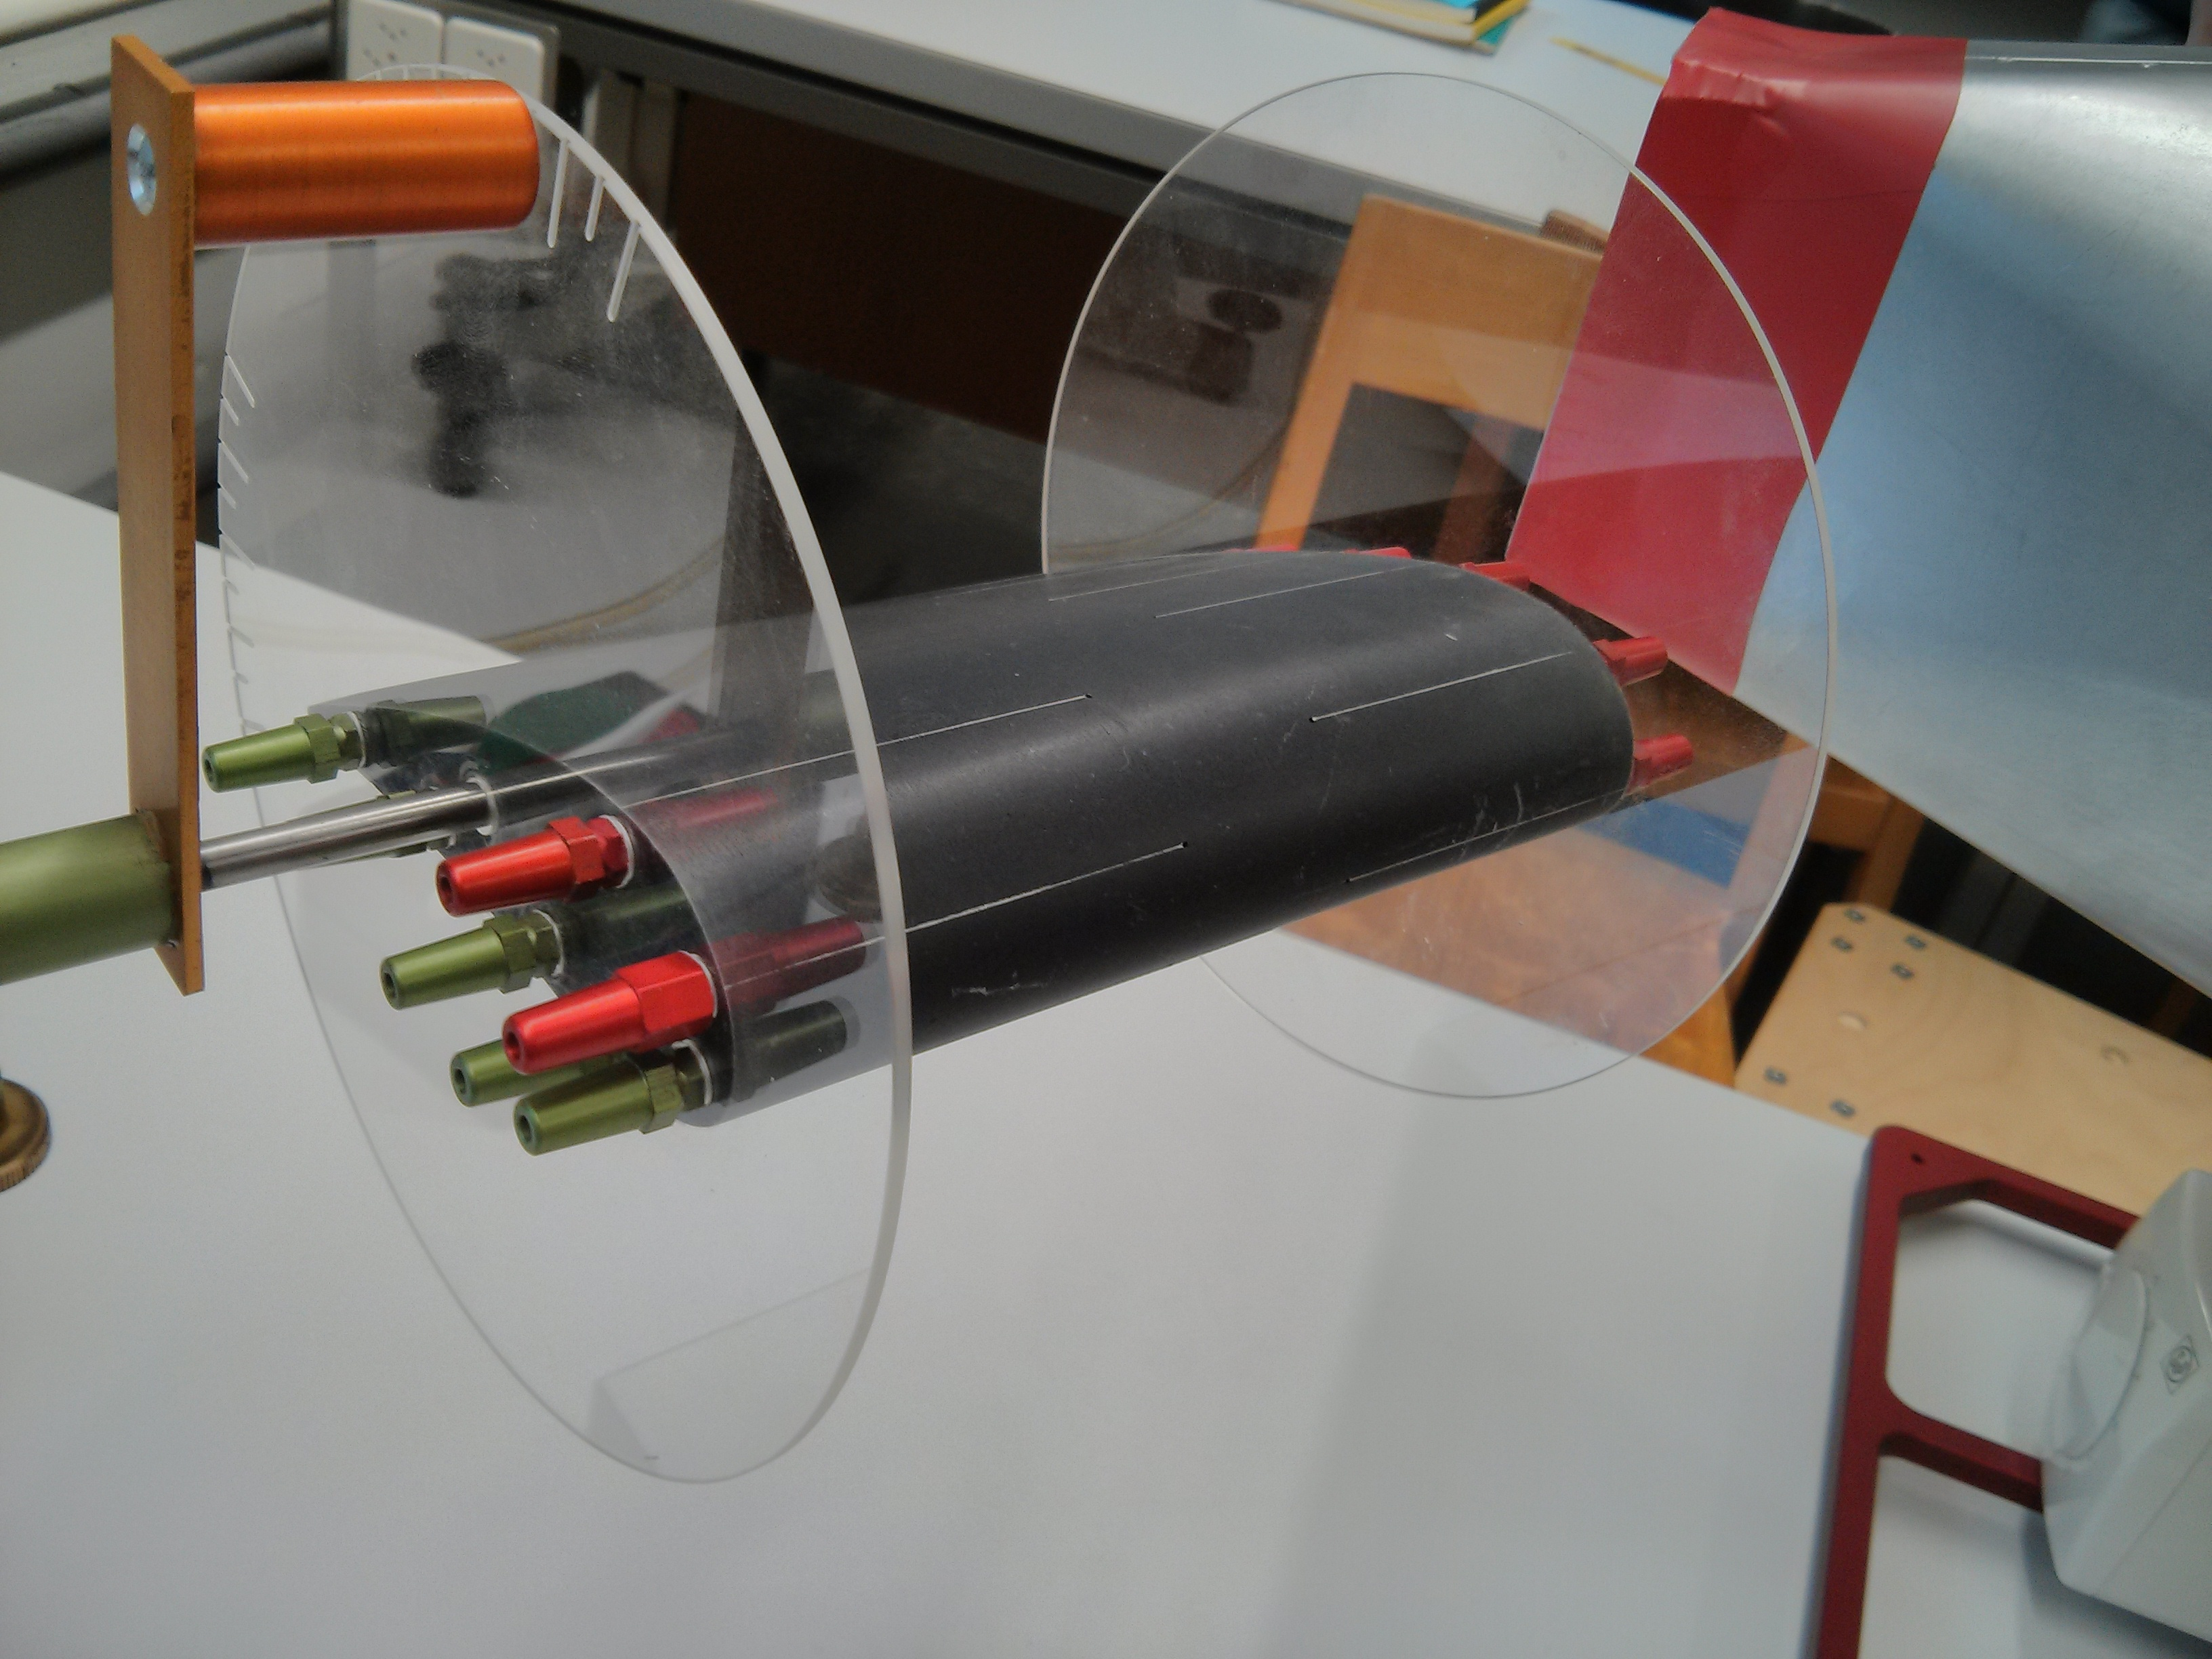
\includegraphics[width=\textwidth]{img/airfoil.jpg}
                \caption{Airfoil}
                \label{fig:airfoil}
        \end{subfigure}%
        ~
        \begin{subfigure}[b]{0.45\textwidth}
                \centering
                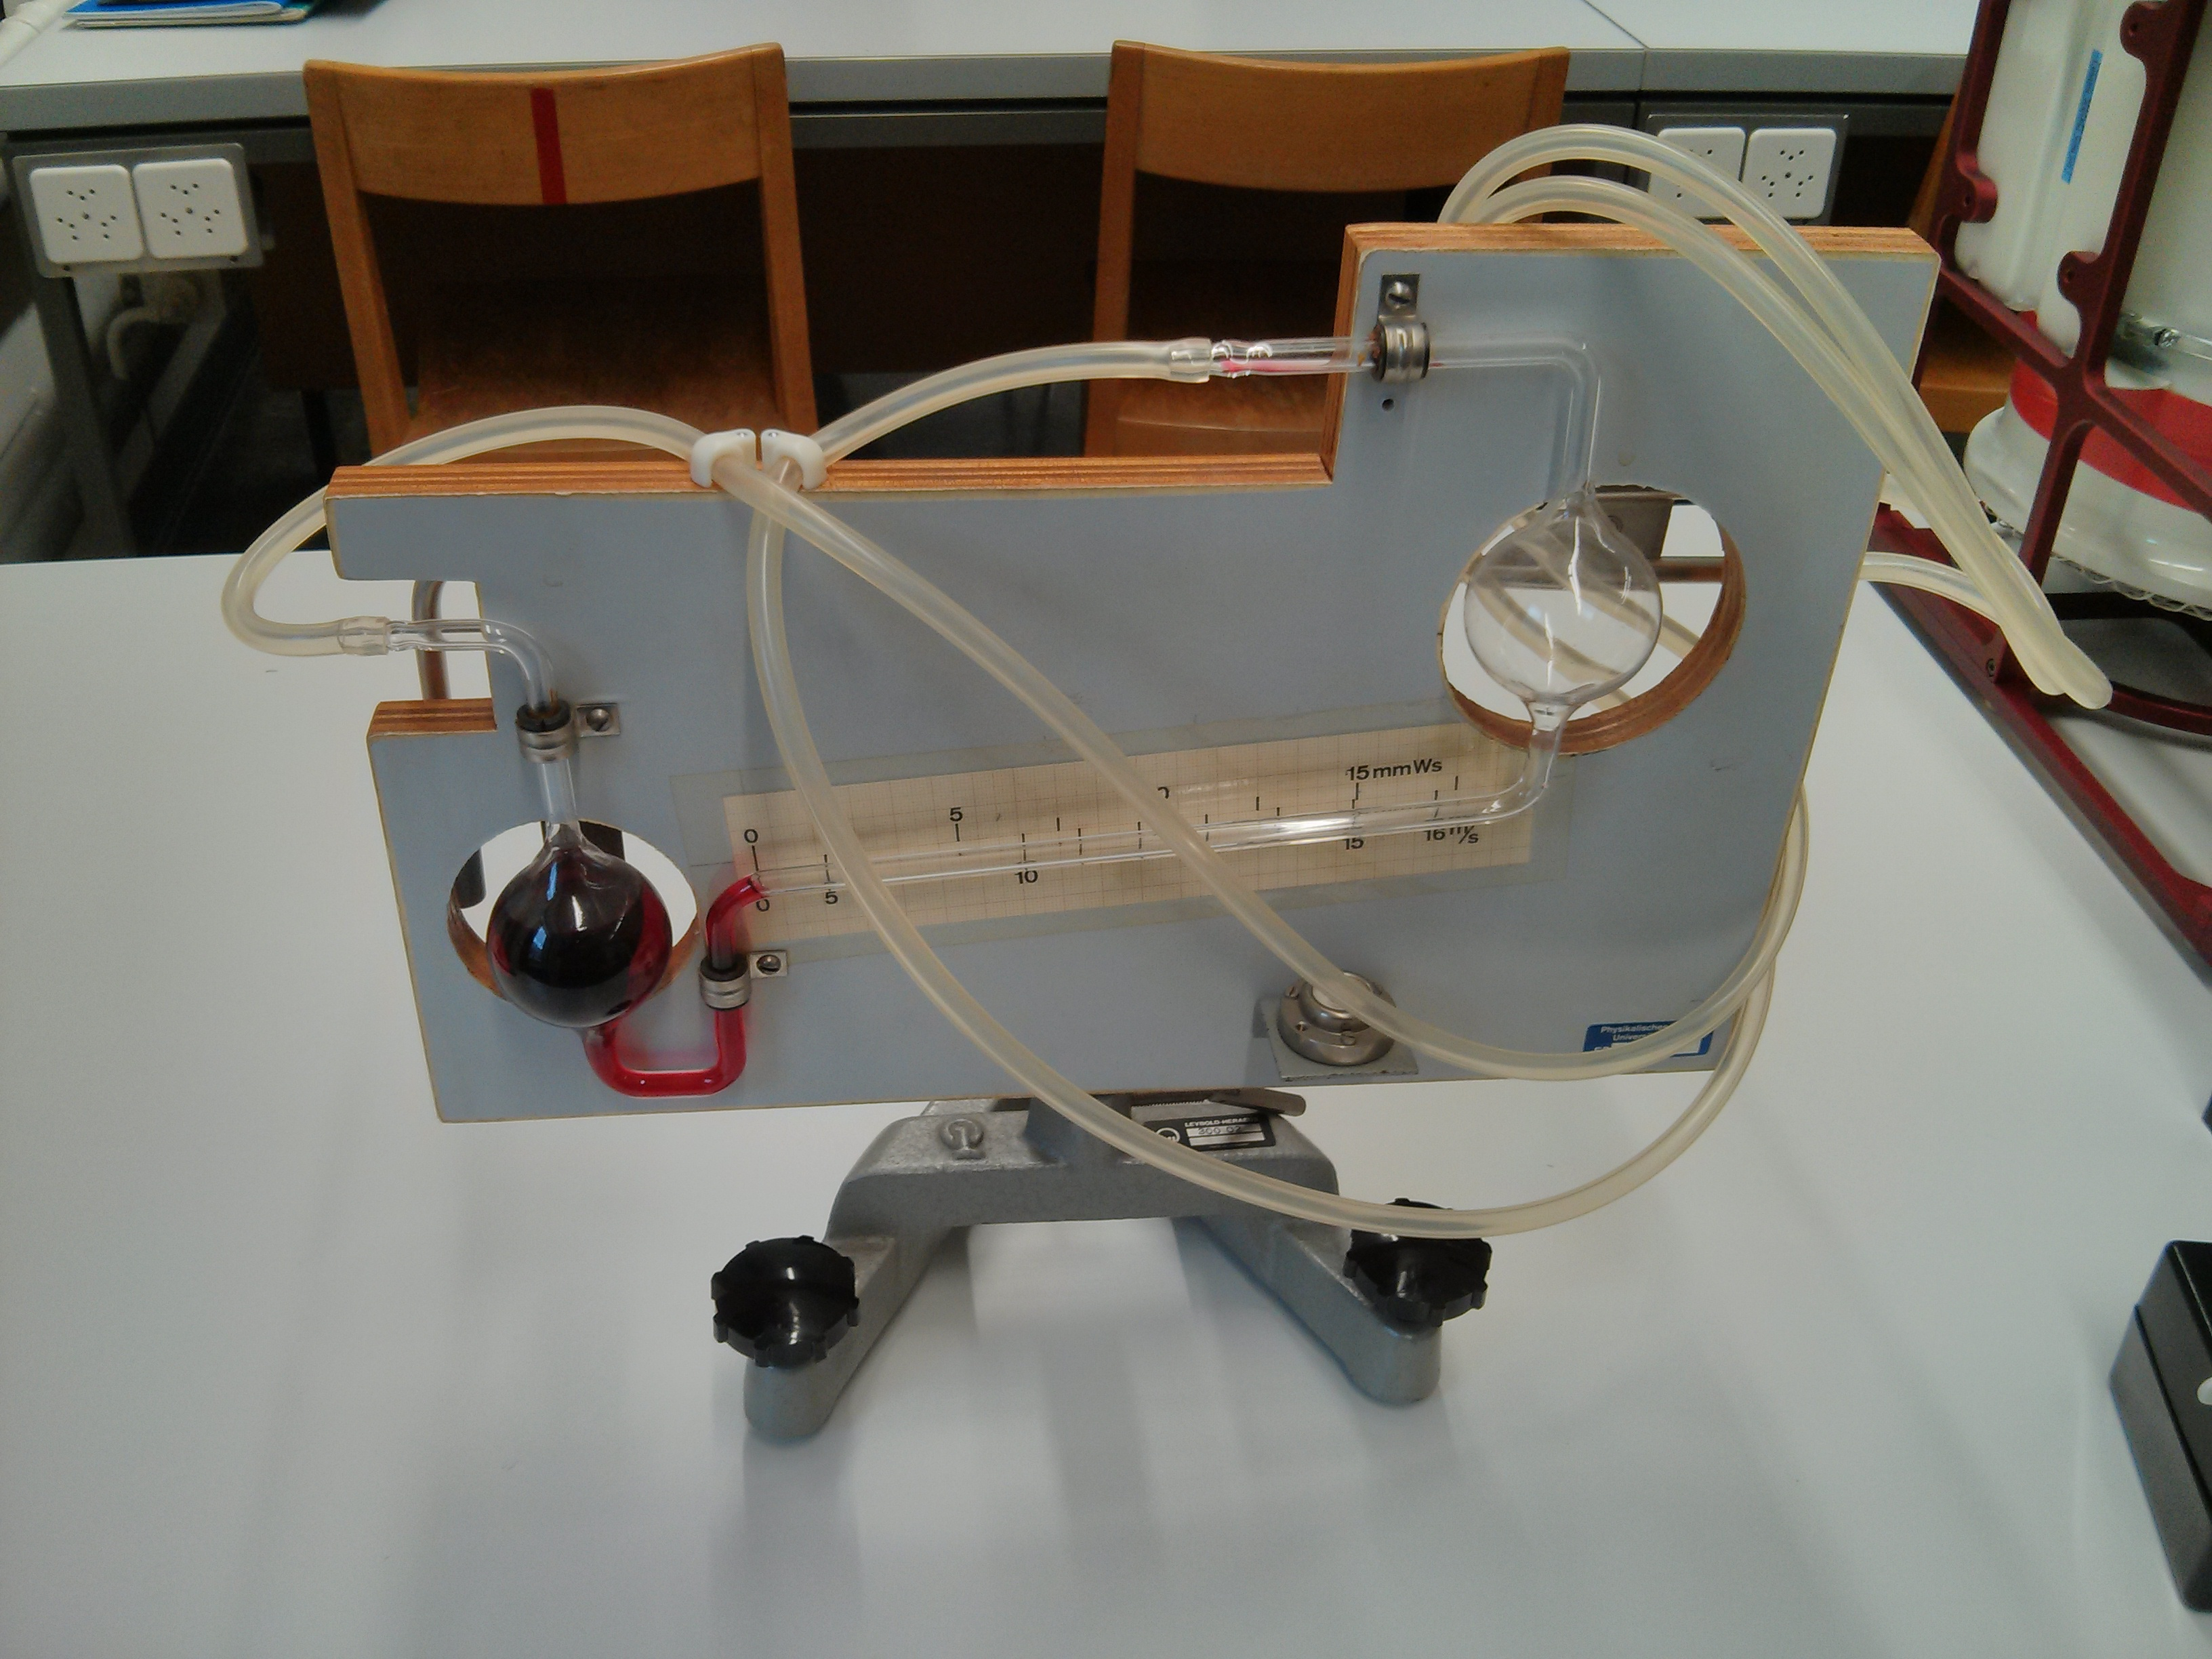
\includegraphics[width=\textwidth]{img/manometer.jpg}
                \caption{Manometer}
                \label{fig:manometer}
        \end{subfigure}
        \caption{Materials used in the experiment}\label{fig:materials}
\end{figure}

\subsection{Assembly}
For this experiment we have to measure three things. And for both of them, we need the wind speed, which is measured using the prandtl tube and left at that value for the whole experiment. Then, we need to measure the air drag of the airfoil at different angles of attack. We do this by arranging the assembly as shown in figure \ref{fig:assembly1}. Now, for every angle between $\ang{-20}$ and $\ang{+20}$ (in $\ang{5}$ steps) the drag is measured using the balance.
Next, we rearrange the assembly as shown in figure \ref{fig:assembly2} and measure the lift for the same angles as before. Last, without modifying the assembly, we proceed to measure the pressure conditions on the surface of the airfoil by attaching a manometer to the foil's holes.

\begin{figure}[H]
	\centering
  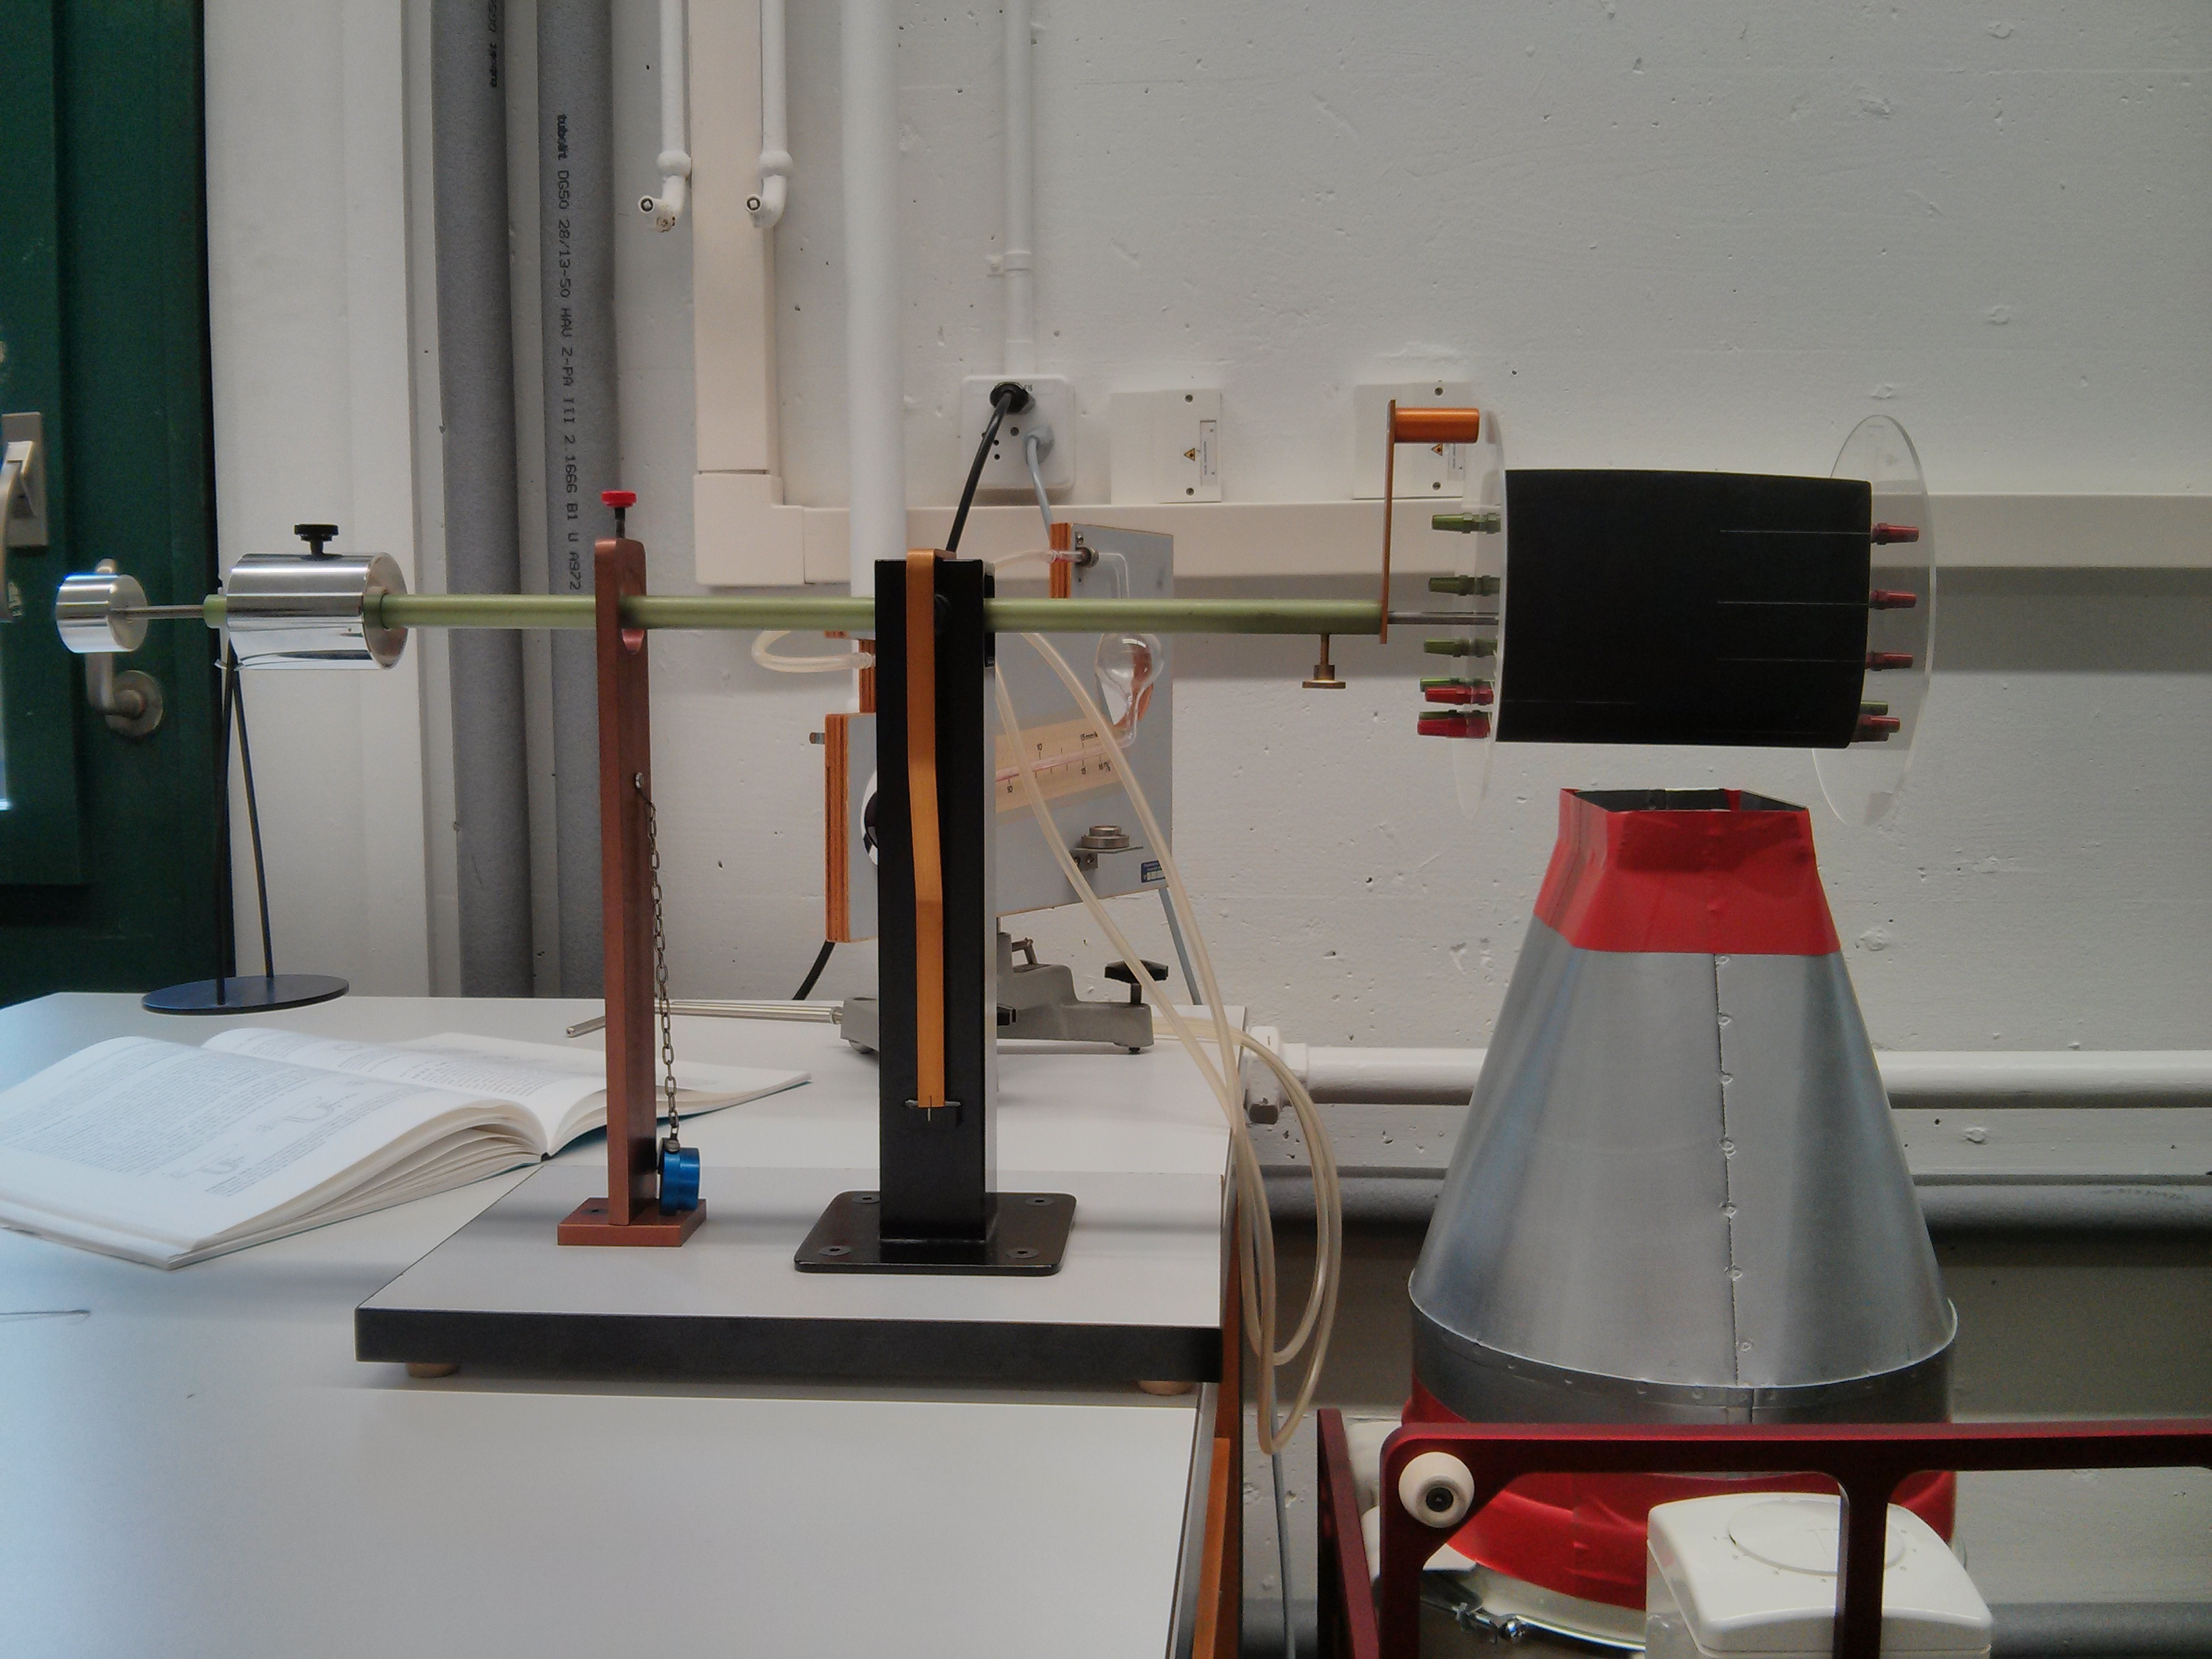
\includegraphics[width=0.9\textwidth]{img/assembly2.jpg}
	\caption{The experiment setup to measure the airfoil's drag $F_r$}
	\label{fig:assembly2}
\end{figure}

\begin{figure}[H]
	\centering
  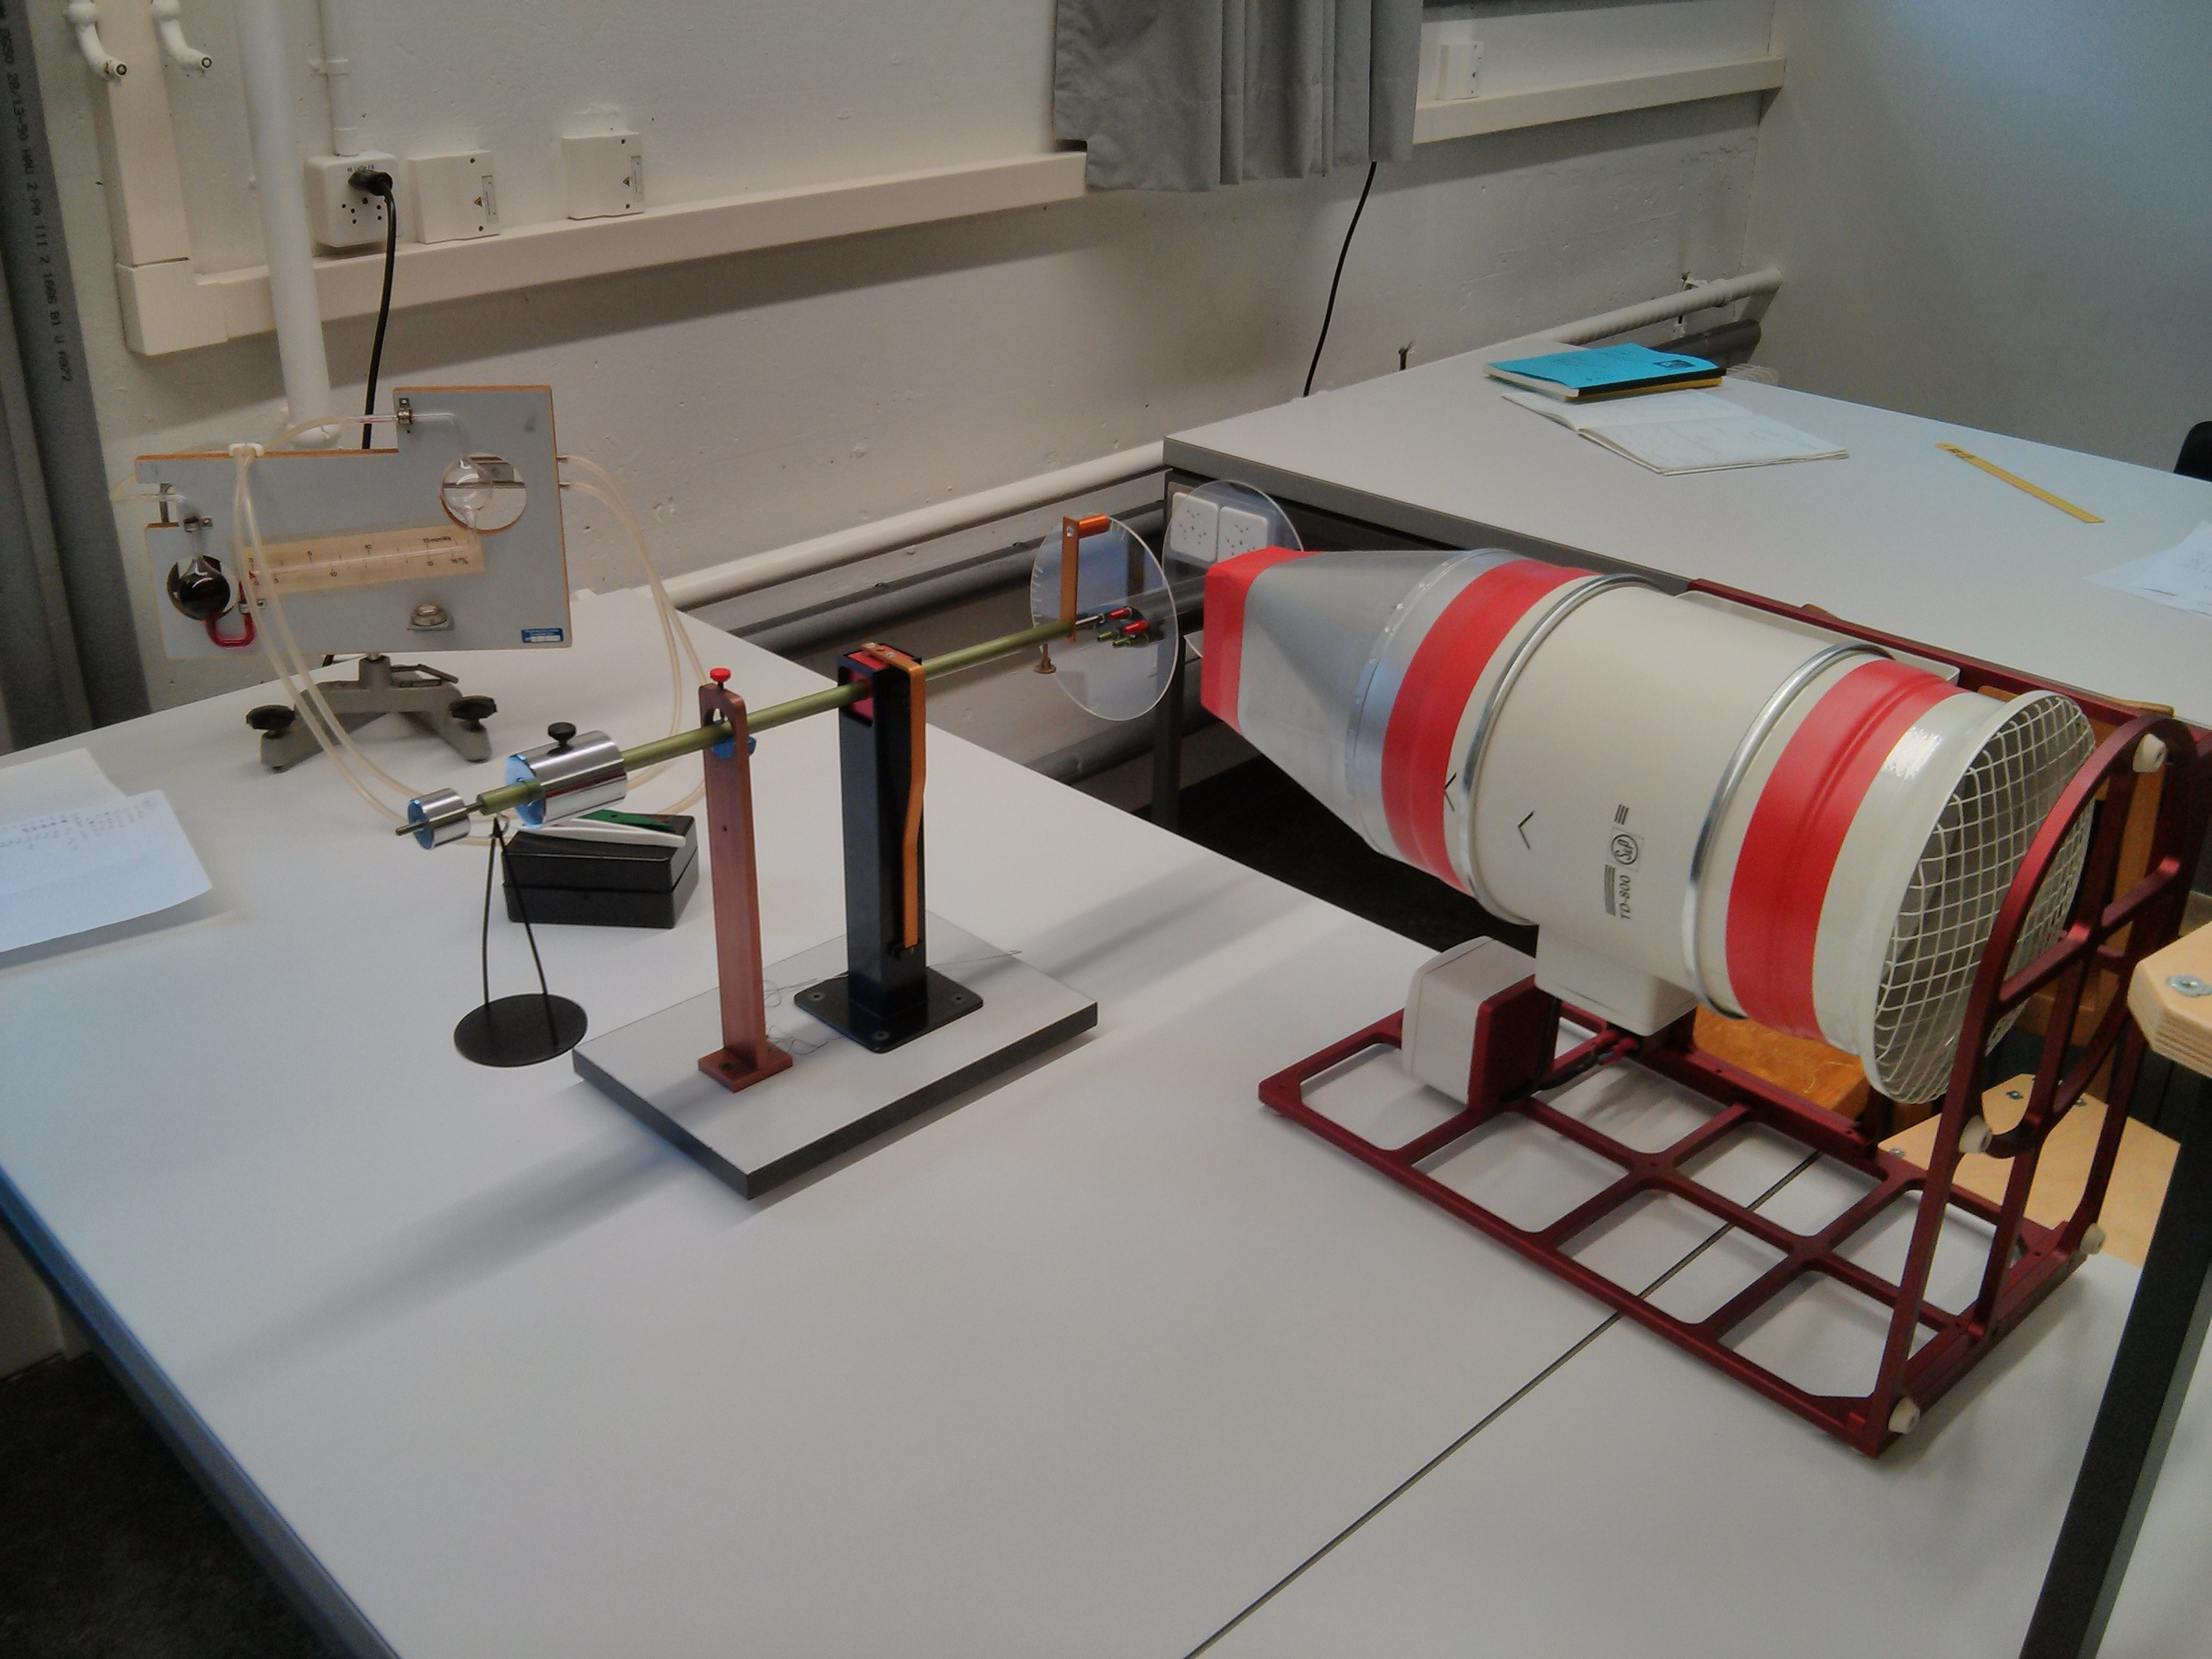
\includegraphics[width=0.9\textwidth]{img/assembly1.jpg}
	\caption{The experiment setup to measure the airfoil's boyant force $F_l$}
	\label{fig:assembly1}
\end{figure}

\section{Measurements}

\subsection{Airfoil Profile}

\begin{figure}[H]
	\centering
  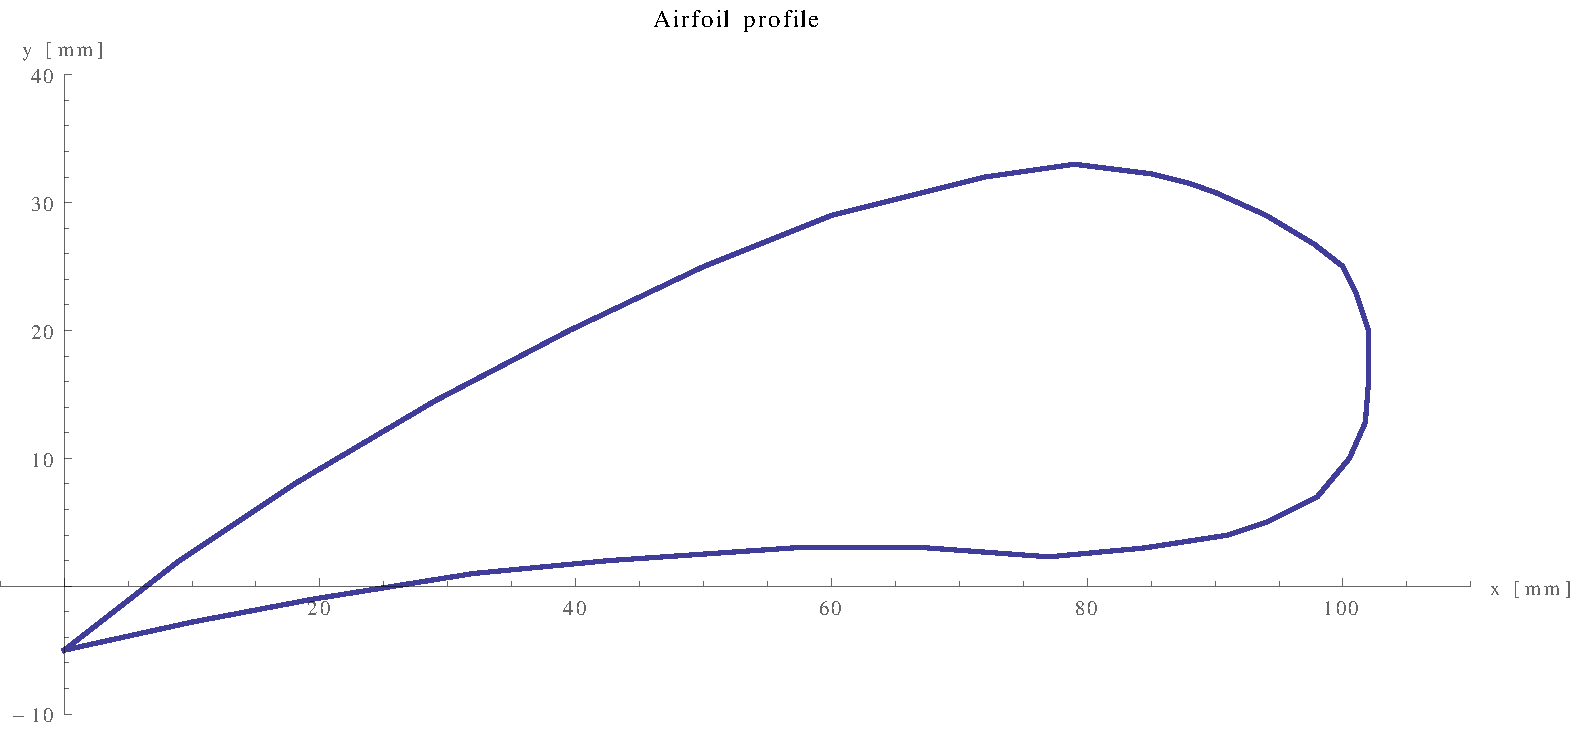
\includegraphics[width=0.9\textwidth]{diag/wing_profile.pdf}
	\caption{Digital representation of the airfoil profile used during the experiment}
	\label{fig:profile}
\end{figure}

\subsection{\boldmath$\lvert F_l\rvert$ and \boldmath$\lvert F_r\rvert$}
In order to calculate $\lvert F_l\rvert$ and $\lvert F_r\rvert$ we used the following masses $m_v$ and $m_h$ to counterbalance the airfoil's air resistance force $F_r$ and boyant force $F_l$ respectively. Some measurements were taken repeatedly after some time for uncertainty analysis.

\begin{table}[H]
\center
\begin{tabular}{|r|c|c|c|c|c|c|c|c|c|}
\hline
Angle & \ang{-20} & \ang{-15} & \ang{-10} & \ang{-5} & \ang{0} & \ang{5} & \ang{10} & \ang{15} & \ang{20}\\
\hline\hline
$m_v$ [g] & 22 & 16.5 & 13 & 12 & 12 & 14 & 16 & 20 & 25\\ 
          & 22 &   -   &  -  &  -  & 12 &  -  &  -  &  -  & 24.5\\ 
          & 22 &   -   &  -  &  -  &  -  & -   & -   &  -  & -\\  
\hline\hline
$m_h$ [g] & 4 & 10 & 16.5 & 23 & 30 & 37 & 42 & 52 & 43\\
& - & - & - & - & - & 35 & - & - & -\\
& - & - & - & - & - & 36 & - & - & -\\
\hline
\end{tabular}
\caption{Measurements of $m_v$ and $m_h$ at different angles of attack}
\label{tab:polarmes}
\end{table}

\subsection{Air pressure around wing profile}
After measuring drag and lift we proceeded to measure the pressure at the below indicated points along the profile of the airfoil.
\begin{figure}[H]
	\centering
  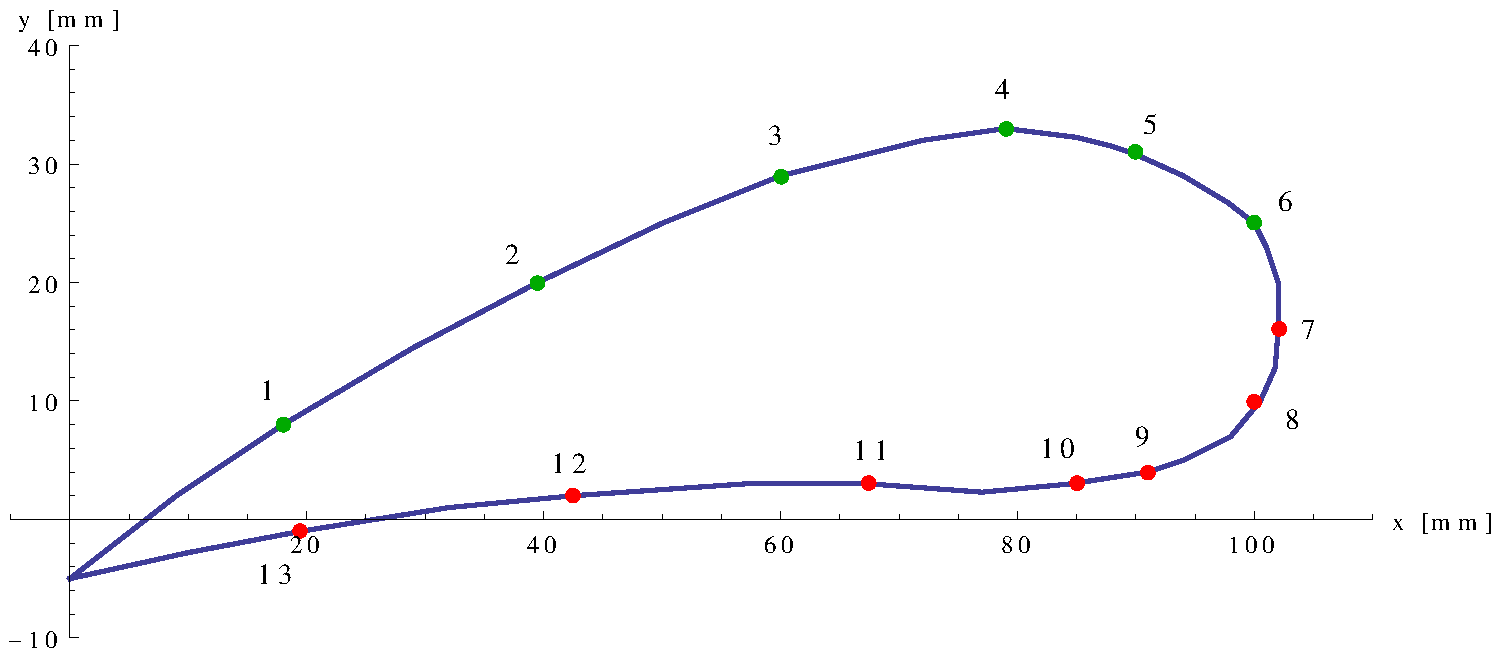
\includegraphics[width=0.9\textwidth]{diag/pressure_points.pdf}
	\caption{Locations at which the pressure was measured. Green points belong to upper data series, red points to lower data series. Rightmost pressure point is used for both data series}
	\label{fig:prespoints}
\end{figure}

\begin{table}[H]
\centering
\begin{tabular}{|r|r|r|}
\hline
Point & \multicolumn{2}{c|}{Pressure}\\
No. &  \multicolumn{2}{c|}{[mmWs]} \\
\hline\hline
1 & -0.1 & -\\
2 & -1.0 & -\\
3 & -5.6 & -\\
4 & -14.6 & -\\
5 & -13.0 & -12.7 \\
6 & 0.5 & -\\
\hline
7 & 15.5 & -\\
\hline
8 & 5.4 & -\\
9 & -8.8 & -\\
10 & -7.5 & -\\
11 & -0.8 & -\\
12 & 2.3 & 2.2\\
13 & 1.5 & -\\
\hline
\end{tabular}
\end{table}

\section{Analysis and Discussion}
\subsection{Polar diagram}
In order to calculate $\lvert F_l\rvert$ and $\lvert F_r\rvert$ we use our measurements in table \ref{tab:polarmes} and the following formulae:
\begin{align}
F_l &= \Delta F_g = m_v \cdot g\\
F_r &= m_h \cdot g
\end{align}
and we can draw the polar diagram accordingly:

\begin{figure}[H]
	\centering
  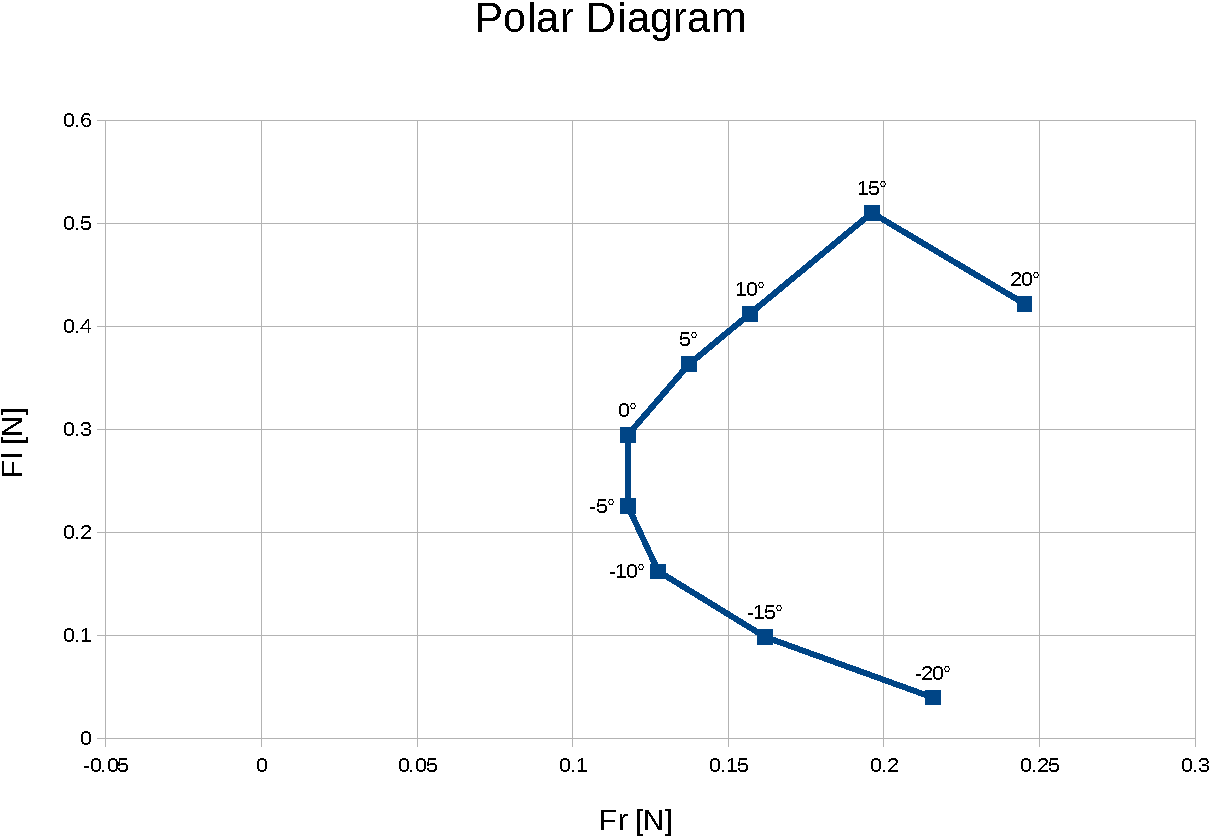
\includegraphics[width=0.9\textwidth]{diag/polar_diag.pdf}
	\caption{The polar diagram obtained by our measurements. $\lvert F_r\rvert$ is indicated along the horizontal axis and $\lvert F_l\rvert$ along the vertical axis at different angles of attack, measured in Newtons [N]}
	\label{fig:poldiag}
\end{figure}



\subsection{Calculating the foil's boyant force $\lvert F_l\rvert$}
\subsubsection{By weighing}
Calculating the foil's boyant force by weighing is very easy. We can just use the values we obtained in table \ref{tab:polarmes}
\begin{figure}[H]
	\centering
  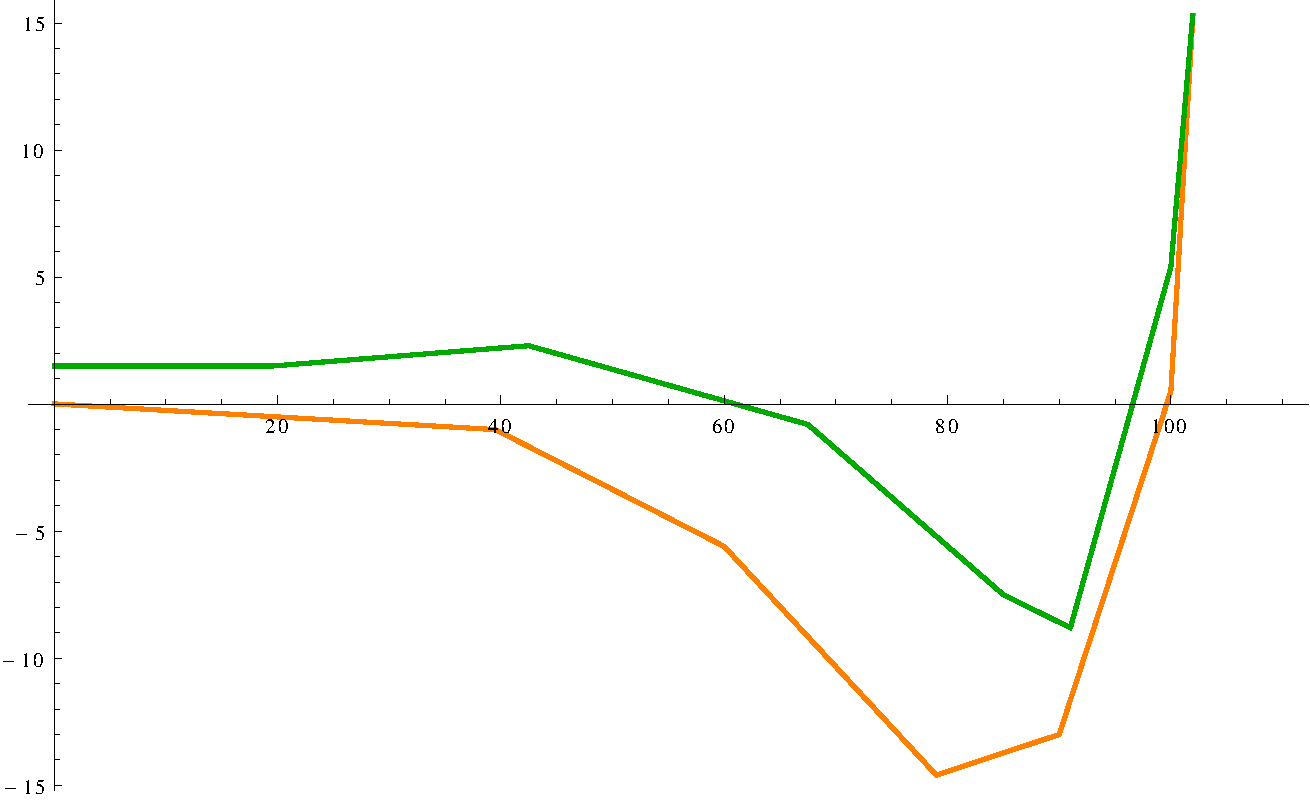
\includegraphics[width=0.9\textwidth]{diag/meas_pressure.pdf}
	\caption{Measured air pressure at predefined measuring points around the airfoil's profile}
	\label{fig:pressure}
\end{figure}

\section{Conclusion}

\begin{thebibliography}{9}

\bibitem{physcript13}
  Peter Wurz,
  \emph{Anleitung zum Physikpraktikum}
  FS2013

\end{thebibliography}

\end{document}
